\section{Systembeskrivelse}

\begin{figure}[H]
\centering
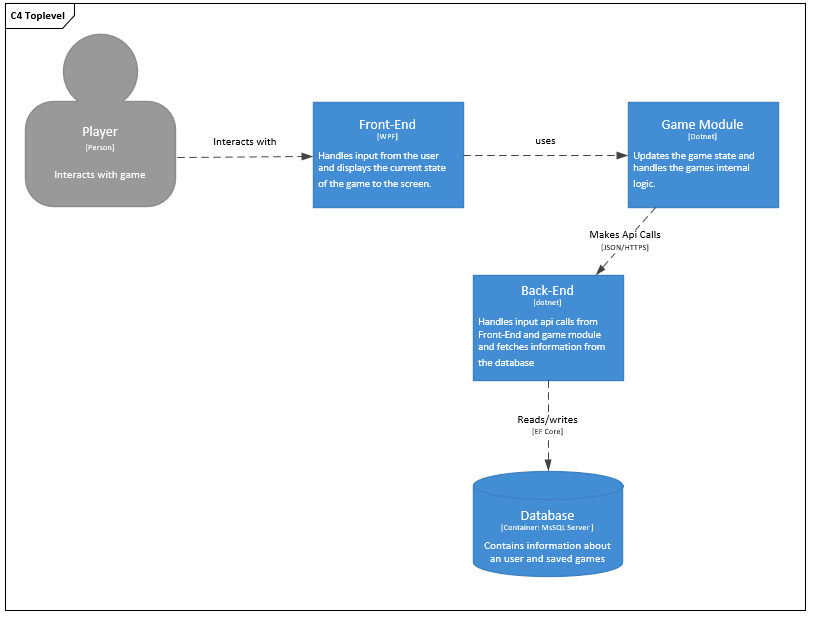
\includegraphics[width = \textwidth]{02-Body/Images/C4TopLvlDB}
\caption{C4 top level diagram, som viser kommunikation mellem systemets segmenter}
\label{fig:C4TopLvlDB}
\end{figure}

På figuren herover ses systemets toplevel arkitektur.
Denne består af en bruger som interagerer med systemet gennem frontendapplikationen som skrives i WPF. States i denne applikation styres af Game modul som holder styr på hvor spilleren befinder sig, hvilke items der er samlet op og andre nyttige information som skal bruges gennem spillet.
Spillets backend benyttes primært til bruger authentication og som bindeled til databasen.
Databasen indeholder oplysninger om blandt andet brugere, de gemte spil og oplysninger om historien for de forskellige rum.



\section{Kravspecifikation}

I det følgende afsnit vil vi uddybe de forudbestemt krav til projektets specifikation. Dette indeholder en systembeskrivelse, samt en accepttestspecifikation til de opsatte krav.
Kravene til systemet vil være opdelt i funktionelle og ikke funktionelle, hvor de opsatte ikke-funktionelle krav vil være prioriteret efter MoSCoW princippet.
Der er ydermere opsat accepttest som tester alle scenarier i de opsatte user stories, samt systemets ikke-funktionelle krav.

\subsection{Funktionelle krav - User Stories}
I dette afsnit forklares systemets funktionelle krav i form af user stories som tager os igennem systemet og de ønskede funktioner. \\
 
User Story 1: Log in \\
  Som Bruger \\
  Kan jeg logge ind \\
  For at kunne se en Main Menu så jeg kan spille spillet. \\
  
User Story 2: Opret profil \\
  Som Bruger \\
  Kan jeg oprette en ny profil \\
  For at jeg kan logge ind på spillet. \\

User Story 3: Main Menu - Settings \\
  Som bruger \\
  Kan jeg tilgå Settings \\
  For at jeg kan customize interfacet \\

User Story 4: Main Menu -- Start Spil \\
  Som bruger \\
  Kan jeg starte et nyt spil \\ 
  Ved at give spillet et navn som bruges til save games \\

User Story 5: Exit game \\
  Som Bruger \\ 
  Kan jeg trykke Esc \\
  For at se en menu med mulighederne "Return to game", "Save and Exit", "Exit without saving" and "Settings". \\

User Story 6: Exit Menu - Resume Game\\
  Som Bruger \\
  Kan jeg trykke på "Resume game" \\
  For at vende tilbage til spillet\\

User Story 7: Exit Menu - Save and Exit\\
  Som Bruger \\
  Kan jeg trykke på "Save and Exit" \\
  For at spillet gemmes og bruger bliver vist Main Menu\\

User Story 8: Exit Menu - Exit Without Saving\\
  Som Bruger \\
  Kan jeg trykke på "Exit Without Saving"\\
  For at få en "Are you Sure" alert\\

User Story 9: Exit Menu - Exit Without Saving - No\\
  Som Bruger\\
  Kan jeg trykke på "No" \\
  For at vende tilbage til exit menu\\

User Story 10: Exit Menu - Exit Without Saving - yes\\
  Som Bruger\\
  Kan jeg trykke på "Yes" \\
  For at vende tilbage til Hovedmenuen uden at gemme\\

UserStory 11 : Exit Menu - Settings\\
  Som Bruger \\
  Kan jeg trykke på "Settings" \\
  For at se Settings Menuen.\\


UserStory 12 : Settings Menu - Efter ændringer\\
  Som bruger \\
  Kan jeg trykke "Apply", "back", "Cancel" og "Default"\\
  For at tilpasse spillets indstillinger\\

UserStory 13 : Settings Menu - Efter ændringer - Apply\\
  Som Bruger \\
  Kan jeg  trykke "Apply" \\
  For at ændre settings\\

UserStory 14 : Settings Menu - Efter ændringer - back\\
  Som Bruger \\
  Kan jeg trykke "back" \\
  For at brugeren sendes tilbage til Esc Menu\\

UserStory 15 : Settings Menu - Efter ændringer - Cancel\\
  Som Bruger \\
  Kan jeg trykke på "Cancel" \\
  For at ændringerne bliver reverted\\

UserStory 16 : Settings Menu - Efter ændringer - Default\\
  Som bruger \\
  Kan jeg trykke på "Default" \\
  For at sætte settings til defaults\\
  
UserStory 17 : Main Menu - Load Game\\
  Som bruger \\
  Kan jeg trykke på "load game" \\
  For at få en liste a save games.\\


UserStory 18 : Main Menu - Load Game - Load\\
  Som bruger \\
  Kan jeg trykke på "load game" \\
  For at komme ind i spillet og fortsætte med at spille det valgte spil\\

UserStory 19 : Main Menu - Load Game - Delete Game\\
  Som bruger \\
  Kan jeg trykke "delete game" \\
  For at game statet bliver slettet fra cloud.\\

UserStory 20 : Main Menu - Load Game - Back\\
  Som bruger \\
  Kan jeg trykke "back" \\
  For at vende tilbage til Main Menu\\
  
UserStory 21 : Spil Spillet - Bevægelse i spil\\
  Som bruger \\
  Kan jeg vælge mellem actioner ved at bruge tallene 0-9 eller piltasterne til at bevæge mig\\
  For at bevæge karakteren i spillet til et andet rum.\\

UserStory 22 : Spil spillet - Enter nyt room\\
  Som bruger \\
  Får jeg en beskrivelse af et rum, når jeg kommer ind i rummet\\
  Så jeg ved hvad jeg kan inteagere med.\\

User Story 23: Spil spillet - Inventory\\
Som bruger\\
Kan jeg trykke på ”Inventory” knappen\\
For at se genstande som jeg besidder\\
  
UserStory 24: Spil spillet - Combat\\
  Som bruger\\
  Kan jeg trykke på "attack" knappen\\
  For at skade fjenden\\

User Story 25: Spil spillet - Combat - flygt\\
Som bruger\\
Kan jeg trykke på ”flee” knappen\\
For at blive rykket tilbage til forrige rum\\
  
UserStory 26: Spil spillet - Inventory\\
  Som bruger\\
  Kan jeg trykke på "Inventory" knappen\\
  For at tilgå karakterens udrustning\\
  
UserStory 27: Spil spillet - Interact\\
  Som bruger\\
  Kan jeg trykke på "interact" knappen\\
  For at interagere med objekter i det nuværende rum\\
  
UserStory 28: Spil Spillet - Level klaret\\
  Som bruger\\
  Kan jeg færdiggøre det sidste rum\\
  For at få en besked om at spillet er fuldført og mulighed for at tilgå Main Menu\\

\subsection{Ikke-funktionelle krav}
I dette afsnit opsættes systemtets ikke-funktionelle krav. Disse er opdelt efter kategori, hvorved der er krav til FURPS modellens forskellige dele. 
Ikke-funktionelle:\\
  GUI:\\
    - GUI'en skal tilbyde valget mellem 3 resolutions\\
    - GUI'en skal kunne være fullscreen\\
    - GUI'en skal kunne være windowed\\

  SOUND:\\
    - Lyden skal kunne justeres mellem 0-100\% relativt til PC'ens lyd niveau.\\

  DATABASE:\\
    - Skal kunne gemme maksimalt 5 save games\\
    - Skal kunne loade et spil indenfor maksimalt 5s\\
    - Skal gemme hvilke genstande man bruger lige nu\\
    - Skal gemme hvor meget liv man har tilbage.\\
    - Skal gemme hvilke fjender man har slået ihjel.\\
    - Skal gemme hvilke puzzles man har løst\\
    - Skal gemme hvilke rum man har været i.\\
    
  GAMEPLAY:\\
    - Spillets kort skal holde styr på hvilke rum man kan komme til for et givet rum.\\
    - Spillets kort skal kun vise de rum som spilleren har været i.\\
    - Spillets kort skal, hvis spilleren har været i alle rum vise alle rum.\\
    
    - Et rum kan have maksimalt 4 forbindelser til andre rum.\\
    - Et rum skal have mindst 1 forbindelse til andre rum.\\
    - Alle Rum skal kunne nås fra ethvert andet rum, måske ikke direkte, men man skal kunne komme dertil.\\
    
    - Spillerens rygsæk skal kunne indeholde alle spillets genstande.\\
    - Spilleren skal have mulighed for at bruge ét våben og én rustning af gangen.\\
    - Spilleren skal have mulighed for at skifte hvilket våben og hvilken rustning der bruges.\\
   
  COMBAT:\\
    - Når spilleren/fjenden prøver at slå, rammer man kun hvis man på sit angreb slår højere end modstanderens rustningsværdi. Dette afgøres af et simuleret 20-sidet terninge kast, hvortil der lægges en værdi til, korresponderende til spilleren/fjendens våben bonusser.\\
    - Hvis spilleren/fjenden rammer, bliver skaden bestemt af et/flere simulerede terningekast, afhængigt af hvilket våben der bruges\\
    - Hvis spilleren, når nul liv inden fjenden, så dør spilleren og spillet er tabt.\\
    - Hvis fjenden, når nul liv inden spilleren, så dør fjenden og spilleren kan nu frit udforske rummet, som fjenden var i.\\
    - Hvis spilleren drikker en livseleksir bliver spillerens nuværende liv sat til fuldt.\\
    - Hvis spilleren/fjenden rammer, bliver skaden bestemt af et/flere simulerede terningekast, afhængigt af hvilket våben der bruges.\\

PERFORMANCE:\\
    - Spillet skal respondere indenfor maksimalt 5s\\
    - Spillet må ikke have mere end én kommando i aktionskøen af gangen\\
  STABILITY:\\
    - MEANTIME BETWEEN FAILURE - 1Time +- 10Min\\
  DOCUMENTATION:\\
    - Spillet skal have en manual/help page til hvordan alting virker.\\
  SECURITY:\\
    - Username skal være mindst 6 characters\\
    - Username skal være unikt\\
    - Password skal være mindst 8 characters\\
    - Password skal have store og små bogstaver\\
    - Password må ikke indeholde username\\

\subsection{MOSCOW krav}
I dette afsnit er de ikke-funktionelle krav fra ovenstående afsnit prioriteret ved hjælp af MoSCow metoden.\\
MUST\\
  - have en GUI\\
  - have en Database\\
  - Have Netværkskommunikation\\
  - Have en serie af sammenhængende rum.\\
  - Have et start og slut rum som ikke er det samme rum.\\
  - Spillet skal kunne gemmes på en Database.\\
  - Skal kunne hente save game fra databasen\\
  - Skal have en authentication system (Accounts)\\
  - Hvert Rum skal bestå af et beskrivende element og en serie af actioner.\\
  - Spillet skal have instillinger.\\
  - Spillet skal have en Character.\\
  - Spillet skal kunne tage imod user input.\\
  - Spillet skal være udviklet til Windows.\\
  - Spillet skal være testbart i.e. skal være designet med testing in mind.\\

SHOULD\\
  - Have Enemies\\
  - Have Items\\
  - Have Combat mechanics\\
  - Have End Screen\\
  - Have Character Stats\\

COULD\\
  - Have Level development\\
  - Have Procedual world\\
  - Have Text Parser\\
  - Have Difficulty\\
  - Have Security\\

WON'T\\
  - Have Graphics\\

\subsection{Accepttest}
I dette afsnit opsættes systemets Accepttest. Disse er opdelt efter kategori, først er der accepttest for User stories, og herefter de ikke funktionelle krav.

\subsubsection{Funktionelle}
\paragraph{Test af User Story 1 - Login}

\textbf{Scenarie - Succesfuld login}

\textit{Givet at brugerens profil er oprettet på databasen og at serveren er oppe.}

\begin{itemize}
  \item Når bruger indtaster sit login(Brugernavn og password)
  \item og trykker "Log in" på UI
  \item Så skifter skærmen til hovedmenu
\end{itemize}

Resultat:\\
Kommentar:\\

\textbf{Scenarie - Fejlet login}

\textit{Givet at brugerens profil er oprettet på databasen og at serveren er oppe.}

\begin{itemize}
  \item Når bruger indtaster et forkert login(Brugernavn og password)
  \item og trykker "Log in" på UI
  \item Så signaleres der om forkert login-oplysninger til bruger
\end{itemize}

Resultat:\\
Kommentar:\\

\paragraph{Test af User Story 2 - Opret profil}

\textbf{Scenarie - Bruger opretter profil}

\textit{Givet at brugerens profil er oprettet på databasen og at serveren er oppe.}

\begin{itemize}
  \item Når bruger vælger at oprette profil
  \item Så gemmes datanene for brugerens profil på databasen
  \item Og skærmen skiftes til log ind skærmen
\end{itemize}

Resultat:\\
Kommentar:\\

\textbf{Scenarie - Bruger opretter samme profil}

\textit{Givet at brugerens profil er oprettet på databasen og at serveren er oppe.}

\begin{itemize}
  \item Når bruger vælger at oprette en allerede-eksisterende profil
  \item Så signaleres der om at profil allerede eksisterer
\end{itemize}

Resultat:\\
Kommentar:\\

\paragraph{Test af User Story 3 og 4 - Main Menu}

\textbf{Scenarie - Tilgå settings}

\textit{Givet at brugeren er logget ind og har adgang til spillet.}

\begin{itemize}
  \item Når bruger trykker settings i UI
  \item Så går spillet til settings menuen
\end{itemize}

Resultat:\\
Kommentar:\\

\textbf{Scenarie - Start spillet}

\textit{Givet at brugeren er logget ind og har adgang til spillet.}

\begin{itemize}
  \item Når bruger trykker "New Game"
  \item Så vises game-interface for brugeren
\end{itemize}

Resultat:\\
Kommentar:\\

\textbf{Scenarie - Exit game}

\textit{Givet at brugeren er logget ind og har adgang til spillet.}

\begin{itemize}
  \item Når bruger trykker "Exit game"
  \item Så lukker spillet
\end{itemize}

Resultat:\\
Kommentar:\\

\paragraph{Test af User Story 5-16 - Exit Menu}

\textbf{Scenarie - Exit spil}

\textit{Givet at brugeren har trykket "New Game"}

\begin{itemize}
  \item Når bruger trykker "Escape" på keyboardet
  \item Så popper et menuvindue op med mulighederne "Resume Game", "Save Game", ”Main Menu" og "Settings"
\end{itemize}

Resultat:\\
Kommentar:\\

\textbf{Scenarie - In game menu - Resume game}

\textit{Givet at brugeren har trykket "New Game" og derefter har trykket "Escape" på keyboard}

\begin{itemize}
  \item Når bruger trykker "Resume Game" i In game menu
  \item Så forsvinder menuvinduet og spillet fortsætter
\end{itemize}

Resultat:\\
Kommentar:\\

\textbf{Scenarie - In game menu - Save -- No Combat}

\textit{Givet at brugeren har trykket "New Game" og derefter har trykket "Escape" på keyboard}

\begin{itemize}
  \item Når bruger trykker på "Save Game" i In game menuen
  \item Så vises save menuen
  \item Og en liste af gemte spil
\end{itemize}

Resultat:\\
Kommentar:\\

\textbf{Scenarie - In game menu - Save -- Combat}

\textit{Givet at brugeren er i combat}

\begin{itemize}
  \item Når bruger trykker "Escape" på keyboarded
  \item Så kan man ikke se en "Save Game" knap i game menuen
\end{itemize}

Resultat:\\
Kommentar:\\

\textbf{Scenarie - In game menu - Main Menu}

\textit{Givet at brugeren har trykket "New Game" og derefter har trykket "Escape" på keyboard}

\begin{itemize}
  \item Når bruger trykker "Main Menu" i In game menu
  \item Så vises hovedmenuen
\end{itemize}

Resultat:\\
Kommentar:\\

\textbf{Scenarie - In game menu - Settings}

\textit{Givet at brugeren har trykket "New Game" og derefter har trykket "Escape" på keyboard}

\begin{itemize}
  \item Når bruger trykker "Settings"
  \item Så åbnes et vindue med mulighed for konfiguration af spil for bruger
\end{itemize}

Resultat:\\
Kommentar:\\

\textbf{Scenarie - Exit menu - Settings - Apply}

\textit{Givet at brugeren har trykket "Settings" og ændret på resolution indstilling}

\begin{itemize}
  \item Når bruger trykker "Apply"
  \item Så ændres indstillinger som brugeren har ændret
\end{itemize}

Resultat:\\
Kommentar:\\

\textbf{Scenarie - Exit menu - Settings - Back}

\textit{Givet at brugeren har trykket "Settings"}

\begin{itemize}
  \item Når bruger trykker "Back"
  \item Så vises In game menuen
\end{itemize}

Resultat:\\
Kommentar:\\

\textbf{Scenarie - Exit menu - Settings - Default}

\textit{Givet at brugeren har trykket "Settings" og har ændret mindst 1 indstlling}

\begin{itemize}
  \item Når bruger trykker "Default"
  \item Så ændres alle indstiliinger tilbage til default settings
\end{itemize}

Resultat:\\
Kommentar:\\

\paragraph{Test af User Story 17 og 18 - Save Menu}

\textbf{Scenarie - Save Menu - Save Game}

\textit{Givet at brugeren har trykket "Save game" fra Settings menu og ikke er i combat.}

\begin{itemize}
  \item Når bruger vælger et gemt spil
  \item Og sætter navnet til det ønskede
  \item Og trykker på "Save Game" knappen
  \item Så genoptages spillet
\end{itemize}

Resultat:\\
Kommentar:\\

\textbf{Scenarie - Save Menu - Back}

\textit{Givet at brugeren har trykket "Save game" fra Settings menu}

\begin{itemize}
  \item Når bruger trykker "Back" i save game menuen
  \item Så vender spillet ilbage til In game menuen
\end{itemize}

Resultat:\\
Kommentar:

\paragraph{Test af User Story 19-22 - Main Menu}

\textbf{Scenarie - Main menu - Load Game}

\textit{Givet at brugeren er logget ind og har adgang til spillet.}

\begin{itemize}
  \item Når bruger trykker "Load game"
  \item Så vises en liste af gemte spil på profilen
\end{itemize}

Resultat:\\
Kommentar:\\

\textbf{Scenarie - Main menu - Load Game - Load}

\textit{Givet at brugeren er logget ind og har adgang til spillet og trykket "Load Game"}

\begin{itemize}
  \item Når bruger vælger et gemt spil
  \item Og trykker "Load Game"
  \item Så loader spillet det gemte spil med det valgte game state
\end{itemize}

Resultat:\\
Kommentar:\\

\textbf{Scenarie - Main menu - Load Game - Back}

\textit{Givet at brugeren er logget ind og har adgang til spillet og trykket "Load Game"}

\begin{itemize}
  \item Når bruger trykker "Back" i load game-menuen
  \item Så vender spillet tilbage til hovedmenuen
\end{itemize}

Resultat:\\
Kommentar:\\

\paragraph{Test af User Story 23-28 - Spil spillet}

\textbf{Scenarie - Spil spillet - Start spillet}

\textit{Givet at brugeren har trykket "New Game"}

\begin{itemize}
  \item Når bruger anvender piltasterne på keyboard eller trykker på knappen på interfacet til at bevæge sig sydpå fra startrummet
  \item Så bevæger brugeren sig ind i rummet "Syd" for det rum de står i
\end{itemize}

Resultat:\\
Kommentar:\\

\textbf{Scenarie - Spil spillet - Enter nyt room}

\textit{Givet at brugeren har trykket "New Game"}

\begin{itemize}
  \item Når bruger går ind i et nyt rum ved brug af keyboard
  \item Så giver UI en beskrivelse af rummet spilleren befinder sig i
\end{itemize}

Resultat:\\
Kommentar:\\

\textbf{Scenarie - Spil spillet - Combat}

\textit{Givet at brugeren møder en fjende i et rum}

\begin{itemize}
  \item Når bruger trykker "Fight!"
  \item Så ruller brugeren et tal mod fjenden om at skade fjenden
  \item Og derefter ruller fjenden et tal om at skade brugeren
\end{itemize}

Resultat:\\
Kommentar:\\

\textbf{Scenarie - Spil spillet - Combat - Flygt}

\textit{Givet at brugeren møder en fjende i et rum}

\begin{itemize}
  \item Når bruger trykker "Flee"
  \item Så flyttes brugeren tilbage til det rum han kom fra
  \item Og får ikke sit mistede liv tilbage igen
\end{itemize}

Resultat:\\
Kommentar:\\

\textbf{Scenarie - Spil spillet - Inventory}

\textit{Givet at brugeren har trykket "New Game"}

\begin{itemize}
  \item Når bruger trykker "Inventory"
  \item Så vises genstande som bruger besidder
\end{itemize}

Resultat:\\
Kommentar:\\

\textbf{Scenarie - Spil spillet - Interact}

\textit{Givet at brugeren har trykket "Start spil" og at der ike er fjender i rummet}

\begin{itemize}
  \item Når bruger trykker "Interact"
  \item Så kan bruger tage potentielle genstande i rummet til brugerens "Inventory"
\end{itemize}

Resultat:\\
Kommentar:\\

\textbf{Scenarie - Spil spillet - Level klaret}

\textit{Givet at brugeren har fuldført det næstsidste rum}

\begin{itemize}
  \item Når bruger bevæger sig ind i sidste rum
  \item Så får bruger en besked om at spillet er klaret og får mulighed for at gå til "Main Menu"
\end{itemize}

Resultat:\\
Kommentar:\\

\subsubsection{Ikke funktionelle}
\textbf{GUI}\\
\begin{table}[H]
\caption{ Ikke funktionelle tests for GUI}
\label{tab:}
\begin{tabular}{|p{3cm}|p{3cm}|p{3cm}|p{3cm}|}
\hline
Beskrivelse & Verificering & Resultat & Kommentar \\
\hline
GUI'en skal tilbyde valget mellem 3 resolutions & Visuel & & \\
\hline
GUI'en skal kunne være fullscreen & Visuel & &\\
\hline
GUI'en skal kunne være windowed & Visuel & & \\
\hline
\end{tabular}
\end{table}

\textbf{SOUND}\\
\begin{table}[H]
\caption{ Ikke funktionelle tests for SOUND}
\label{tab:}
\begin{tabular}{|p{3cm}|p{3cm}|p{3cm}|p{3cm}|	}
\hline
Beskrivelse & Verificering & Resultat & Kommentar \\
\hline
Lyden skal kunne justeres mellem 0-100\% relativt til PC'ens lyd niveau. & Auditorisk/Visuel & & \\
\hline
\end{tabular}
\end{table}

\textbf{DATABASE}\\
\begin{table}[H]
\caption{ Ikke funktionelle tests for DATABASE}
\label{tab:}
\begin{tabular}{|p{3cm}|p{3cm}|p{3cm}|p{3cm}|}
\hline
Beskrivelse & Verificering & Resultat & Kommentar \\
\hline
Skal kunne gemme maksimalt 5 save games & Visuel & & \\
\hline
Skal kunne loade et spil indenfor maksimalt 5s & Visuel & &\\
\hline
Skal gemme hvilke genstande man bruger lige nu & Visuel & & \\
\hline
Skal gemme hvor meget liv man har tilbage. & Visuel & & \\
\hline
Skal gemme hvilke fjender man har slået ihjel. & Visuel & & \\
\hline
Skal gemme hvilke puzzles man har løst & Visuel & & \\
\hline
Skal gemme hvilke rum man har været i. & Visuel & & \\
\hline
\end{tabular}
\end{table}

\textbf{GAMEPLAY}\\
\begin{table}[H]
\caption{ Ikke funktionelle tests for GAMEPLAY}
\label{tab:}
\begin{tabular}{|p{3cm}|p{3cm}|p{3cm}|p{3cm}|}
\hline
Beskrivelse & Verificering & Resultat & Kommentar \\
\hline
Spillets kort skal holde styr på hvilke rum man kan komme til for et givet rum. & Visuel & & \\
\hline
Spillets kort skal kun vise de rum som spilleren har været i. & Visuel & &\\
\hline
Spillets kort skal, hvis spilleren har været i alle rum vise alle rum. & Visuel & & \\
\hline
Et rum kan have maksimalt 4 forbindelser til andre rum. & Visuel & & \\
\hline
Et rum skal have mindst 1 forbindelse til andre rum. & Visuel & & \\
\hline
Alle Rum skal kunne nås fra ethvert andet rum, måske ikke direkte, men man skal kunne komme dertil. & Visuel & & \\
\hline
Spillerens rygsæk skal kunne indeholde alle spillets genstande. & Visuel & & \\
\hline
Spilleren skal have mulighed for at bruge ét våben og et skjold af gangen. & Visuel & & \\
\hline
Spilleren skal have mulighed for at skifte hvilket våben og hvilket skjold der bruges. & Visuel & & \\
\hline
\end{tabular}
\end{table}

\textbf{COMBAT}\\
\begin{table}[H]
\caption{ Ikke funktionelle tests for COMBAT}
\label{tab:}
\begin{tabular}{|p{3cm}|p{3cm}|p{3cm}|p{3cm}|}
\hline
Beskrivelse & Verificering & Resultat & Kommentar \\
\hline
Når spilleren/fjenden prøver at slå, rammer man kun hvis man på sit angreb slår højere end modstanderens rustningsværdi. Dette afgøres af et simuleret 20 sidet terninge kast, hvortil der lægges en værdi til, korresponderende til spilleren/fjendens våben bonusser. & Visuel & & \\
\hline
Hvis spilleren/fjenden rammer, bliver skaden bestemt af et/flere simulerede terningekast, afhængigt af hvilket våben der bruges. & Visuel & &\\
\hline
Hvis spilleren/fjenden rammer, bliver skaden bestemt af et flere simulerede terningekast, afhængigt af hvilket våben der bruges.  & Visuel & & \\
\hline
Hvis spilleren, når nul liv inden fjenden, så dør spilleren og spillet er tabt. & Visuel & & \\
\hline
Hvis fjenden, når nul liv inden spilleren, så dør fjenden og spilleren kan nu frit udforske rummet, som fjenden var i. & Visuel & & \\
\hline
Hvis spilleren drikker en livseleksir bliver spillerens nuværende liv sat til fuldt & Visuel & & \\
\hline
\end{tabular}
\end{table}

\textbf{PERFORMANCE}\\
\begin{table}[H]
\caption{ Ikke funktionelle tests for PERFORMANCE}
\label{tab:}
\begin{tabular}{|p{3cm}|p{3cm}|p{3cm}|p{3cm}|}
\hline
Beskrivelse & Verificering & Resultat & Kommentar \\
\hline
 Spillet skal respondere indenfor maksimalt 5s & Visuel & & \\
\hline
 Spillet må ikke have mere end én kommando i aktionskøen af gangen & Visuel & &\\
\hline
\end{tabular}
\end{table}

\textbf{STABILITY}\\
\begin{table}[H]
\caption{ Ikke funktionelle tests for STABILITY}
\label{tab:}
\begin{tabular}{|p{3cm}|p{3cm}|p{3cm}|p{3cm}|}
\hline
Beskrivelse & Verificering & Resultat & Kommentar \\
\hline
 MEANTIME BETWEEN FAILURE 1Time + 10Min? & Visuel & & \\
\hline
\end{tabular}
\end{table}

\textbf{DOCUMENTATION}\\
\begin{table}[H]
\caption{ Ikke funktionelle tests for DOKUMENTATION}
\label{tab:}
\begin{tabular}{|p{3cm}|p{3cm}|p{3cm}|p{3cm}|}
\hline
Beskrivelse & Verificering & Resultat & Kommentar \\
\hline
Spillet skal have en manual/help page til hvordan alting virker. & Visuel & & \\
\hline
\end{tabular}
\end{table}

\textbf{SECURITY}\\
\begin{table}[H]
\caption{ Ikke funktionelle tests for SECURITY}
\label{tab:}
\begin{tabular}{|p{3cm}|p{3cm}|p{3cm}|p{3cm}|}
\hline
Beskrivelse & Verificering & Resultat & Kommentar \\
\hline
 Username skal være mindst 6 characters & Visuel & & \\
\hline
 Username skal være unikt & Visuel & & \\
\hline
 Password skal være mindst 8 characters & Visuel & & \\
\hline
 Password skal have store og små bogstavers & Visuel & & \\
\hline
 Password må ikke indeholde username & Visuel & & \\
\hline
\end{tabular}
\end{table}


